\documentclass[11pt,a4paper]{article}
\usepackage[utf8]{inputenc}
\usepackage[german]{babel}
\usepackage{amsmath}
\usepackage{amsfonts}
\usepackage{subfig}
\usepackage{amssymb}
\usepackage{siunitx,physics}
\usepackage{mathtools}
\usepackage{graphicx}
%\usepackage{Here}
\usepackage[version=4]{mhchem}
\usepackage{url}
\usepackage{setspace}
\usepackage[left=2.5cm,right=2.5cm,top=2.5cm,bottom=2cm]{geometry}
[biblography=totocnumbered]
\usepackage{fancyhdr}
\usepackage{scrextend}
\usepackage{hyperref}
\pagenumbering{gobble}

\makeatletter
\newcommand\bigcdot{\mathpalette\bigcdot@{.5}}
\newcommand\bigcdot@[2]{\mathbin{\vcenter{\hbox{\scalebox{#2}{$\m@th#1\bullet$}}}}}
\makeatother

\makeatletter
%\renewcommand*\bib@heading{%
%  \subsection*{}%
%  \@mkboth{\refname}{\refname}}
%\makeatother
\numberwithin{equation}{section}
\numberwithin{figure}{section}

\renewcommand{\labelitemii}{\labelitemfont$\vartriangleright$}
\begin{document}\\
\begin{addmargin}[25pt]{0pt}
\begin{figure}[h]
    \centering
    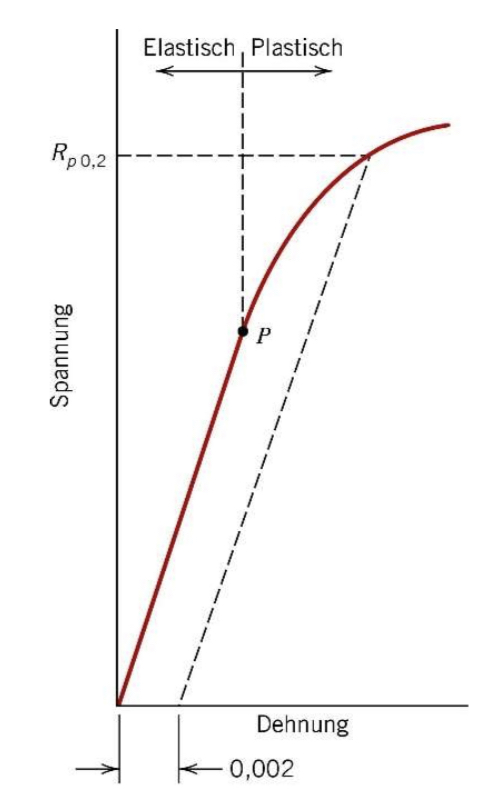
\includegraphics[width=0.5\textwidth]{images/Materialwissenschaften/plastische_Verformung.jpeg}
    \caption{Vergleich von elastischem und plastischem Bereich }
    \label{fig:plastische_Verformung}
\end{figure}
Bei sehr großen Dehnungen werden die Kristallstrukturen stark genug auseinander gezogen dass Bindungen reißen können, diesen Bereich nennt man Bereich der plastischen Verformung. Da einige Bindungen nun aufgebrochen sind ist der Widerstand des Werkstoffs gegenüber Verformung nicht mehr so stark und die Spannungs-Dehnungs-Kurve steigt flacher an als im elastischen Bereich (siehe Abbildung \ref{fig:plastische_Verformung}). Der Spannungswert ab dem es zu plastsischer Verformung kommt nennt sich Streckgrenze. Außerdem kann man die Ersatzstreckgrenze definieren, das ist die Spannung die sich aus dem Schnittpunkt der Spannungs-Dehnungs-Kurve mit einer zum linearen Bereich parallelen Gerade, welche bei $\epsilon = 0,002$ die Dehnungs-Achse schneidet, ergibt.\\
\end{addmargin}

\end{document}